\documentclass[11]{article}
\usepackage[margin=1in]{geometry}
\usepackage{amsmath,amssymb,amsthm,enumitem}
\usepackage{fullpage}
\usepackage{tikz}
\usepackage[latin1]{inputenc}
\usetikzlibrary{arrows,shapes.gates.logic.US,shapes.gates.logic.IEC,calc,trees}
\usepackage{xcolor}
\usepackage{listings}

\definecolor{comment}{rgb}{0.0, 0.5, 0.0}

\lstdefinestyle{CStyle}{
    backgroundcolor=\color{lightgray},   
    commentstyle=\color{comment},
    keywordstyle=\color{blue},
    numberstyle=\tiny\color{black},
    stringstyle=\color{violet},
    basicstyle=\footnotesize,
    breakatwhitespace=false,         
    breaklines=true,                 
    captionpos=b,                    
    keepspaces=true,                 
    numbers=left,                    
    numbersep=5pt,                  
    showspaces=false,                
    showstringspaces=false,
    showtabs=false,                  
    tabsize=2,
    language=C
}

\begin{document}

\tikzstyle{branch}=[fill,shape=circle,minimum size=3pt,inner sep=0pt]

\begin{titlepage}
\begin{center}
\vspace*{2cm}
\Large{\textbf{EECE 5643: Simulation and Performance Evaluation}}\\
\Large{\textbf{Professor Ningfang Mi}}\\
\vfill
\line(1,0){400}\\[1mm]
\huge{\textbf{Homework 2}}\\[3mm]
\Large{\textbf{- Assignment Due: 02/06/2023 -}}\\[1mm]
\line(1,0){400,0}\\
\vfill
Harrison Sun\\
Monday, Thursday 11:45 am - 1:25 pm \\
Completed: \today\
\end{center}
\end{titlepage}

\section{\textbf{Ex. 1.2.2}}
\textbf{(a) Modify program $ssq1$ by adding the capability to compute (1) the maximum
delay, (2) the number of jobs in the service node at a specified time (known at a compile time), and (3) the proportion of jobs delayed.\\\\}

\begin{lstlisting}[style=CStyle]

/**
 * Modified February 4, 2023 by hlsun
 * sun.har@northeastern.edu
 * 
 * Added            : Calculations for (1) Maximum Delay, (2) Number of jobs at a given time, (3) Proportion of jobs delayed.
 * Changed          : Changed language from C to C++. Changed to use terminal arguments.
 * Compile with     : g++ -Wall -o Homework2.1 Homework2.1.cpp
 */


/* -------------------------------------------------------------------------
 * This program simulates a single-server FIFO service node using arrival
 * times and service times read from a text file.  The server is assumed
 * to be idle when the first job arrives.  All jobs are processed completely
 * so that the server is again idle at the end of the simulation.   The
 * output statistics are the average interarrival time, average service
 * time, the average delay in the queue, and the average wait in the service 
 * node. 
 *
 * Name              : ssq1.c  (Single Server Queue, version 1)
 * Authors           : Steve Park & Dave Geyer
 * Language          : ANSI C
 * Latest Revision   : 9-01-98
 * Compile with      : gcc ssq1.c 
 * ------------------------------------------------------------------------- 
 */

#include <stdio.h>   
#include <stdlib.h> 

#define FILENAME    "ssq1.dat"                  /* input data file */
#define TIMESET     400.0                       /* time at which number of jobs in the service node is calculated */
#define START       0.0

/* =========================== */
    double GetArrival(FILE *fp)                 /* read an arrival time */
/* =========================== */
{ 
    double a;

    fscanf(fp, "%lf", &a);
    return (a);
}

/* =========================== */
    double GetService(FILE *fp)                 /* read a service time */
/* =========================== */
{ 
    double s;

    fscanf(fp, "%lf\n", &s);
    return (s);
}

/* ============== */
    int main(int argc, char* argv[])
/* ============== */
{
    FILE   *fp;                                  /* input data file      */
    long   index     = 0;                        /* job index            */
    double arrival   = START;                    /* arrival time         */
    double delay;                                /* delay in queue       */
    double service;                              /* service time         */
    double wait;                                 /* delay + service      */
    double departure = START;                    /* departure time       */
    struct {                                     /* sum of ...           */
    double delay;                              /*   delay times        */
    double wait;                               /*   wait times         */
    double service;                            /*   service times      */
    double interarrival;                       /*   interarrival times */
    } sum = {0.0, 0.0, 0.0};

    double MaxDelay = 0;                         /* This variable stores the maximum delay.  */
    int numJobsAtT = 0;                          /* This variable stores the number of jobs at a given time. */
    int timeT = (int) TIMESET;                   /* This variable stores the time at which to calculate numJobsAtT. */
    int numJobsDelayed = 0;                      /* This variable stores the number of jobs delayed. */

	/* If filename is specified as a terminal argument, use that. Else, use the default filename. */
	fp = (argc > 1) ? fopen(argv[1], "r") : fopen(FILENAME, "r");
    
	/* If time is specified as a terminal argument, use that. Else, use the default time. */
	timeT = (argc > 2) ? atoi(argv[2]) : timeT;

    if (fp == NULL) {
    fprintf(stderr, "Cannot open input file %s\n", FILENAME);
    return (1);
    }

    while (!feof(fp)) {
    index++;
    arrival      = GetArrival(fp);
    if (arrival < timeT)
		numJobsAtT++;   /* Increment the number of jobs if it arrives before timeT */
    if (arrival <= departure)
    {
        delay = departure - arrival;        /* delay in queue    */
		numJobsDelayed++;                   /* Increment the number of jobs delayed. */
    }
    else 
        delay      = 0.0;                        /* no delay          */
    service      = GetService(fp);
    wait         = delay + service;
    departure    = arrival + wait;             /* time of departure */
	if (departure <= timeT)
		numJobsAtT--;   /* Decrement the number of jobs if it departs before timeT */
    sum.delay   += delay;
    sum.wait    += wait;
    sum.service += service;
    /* If the delay is greater than the previous maximum delay, store it as MaxDelay. */
    if (delay > MaxDelay)
    {
        MaxDelay = delay;
    }
    }
    sum.interarrival = arrival - START;

    printf("\nfor %ld jobs\n", index);
    printf("   average interarrival time \t= \t%6.2f\n", sum.interarrival / index);
    printf("   average service time .... \t= \t%6.2f\n", sum.service / index);
    printf("   average delay ........... \t= \t%6.2f\n", sum.delay / index);
    printf("   average wait ............ \t= \t%6.2f\n", sum.wait / index);

    printf("   maximum delay ........... \t= \t%6.2f\n", MaxDelay);
    printf("   number of jobs at t = %d  \t= \t%6.1d\n", timeT, numJobsAtT);
    printf("   proportion of jobs delayed\t= \t%6.2f\n", (double) numJobsDelayed / index);

    fclose(fp);
    return (0);
}

\end{lstlisting}
\vspace{20pt}
\noindent Terminal Output:\\\\

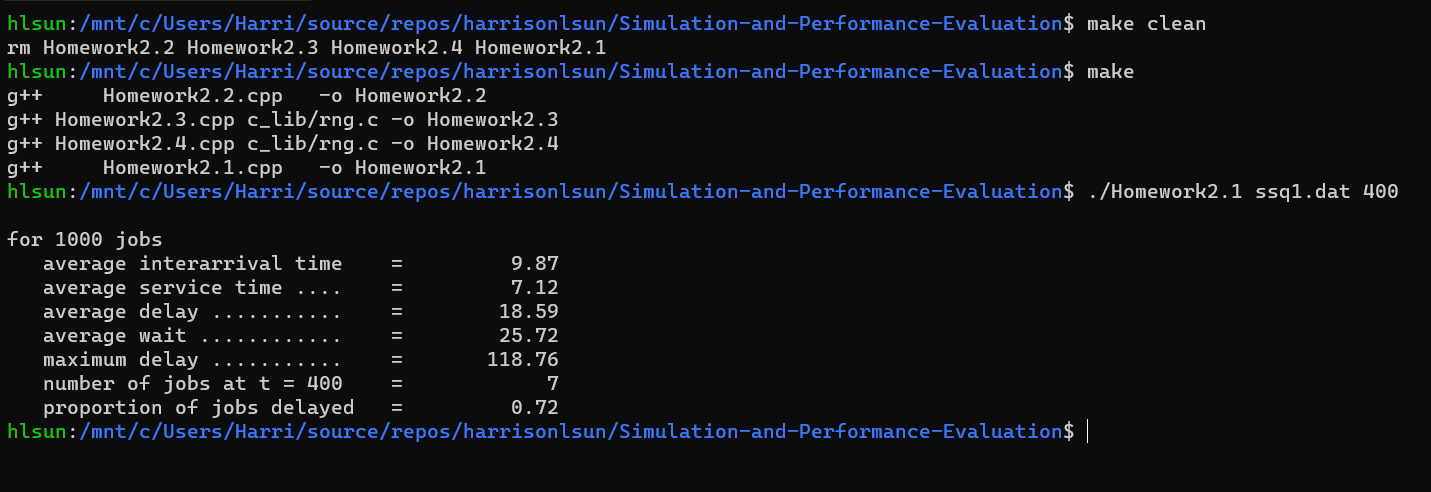
\includegraphics[scale = 0.5]{Sections/H2_1.png}
\newpage

\noindent\textbf{(b) What was the maximum delay experienced?\\\\}
The maximum delay experienced was 118.76.\\\\
\textbf{(c) How many jobs were in the service node at t=400, and how does the computation of this number related to the proof of Theorem 1.2.1?\\\\}
There were 7 jobs in the service node at t=400. This relates to the proof of Theorem 1.2.1 in that the departure time of the job is related to the arrival time such that it is equal to the sum of the arrival time, delay time, and service time. In the case where the service node is empty at the arrival time, the delay time is 0. When the arrival event occurs, we can say that the number of jobs in the service node increments by 1. Similarly, when a departure event occurs, we can say that the number of jobs in the service node decrements by 1. Thus, the number of jobs in the node at any given time is equal to the number of jobs that arrived subtracted by the number of jobs that have left the service node up the the specified time. That is, the number of jobs in the service node is equal to the number of jobs currently being processed plus the number of jobs waiting in the queue.\\\\ 
\textbf{(d) What proportion of jobs were delayed and how does the proportion related to the utilization?\\\\}
72\% of jobs were delayed. This is related to the utilization in that having jobs waiting to start after the previous job is completed increases the utilization because there is no time in between where the server is idle. However, the proportion of jobs that are delayed is not necessarily proportional to the utilization, as the service time of the jobs may differ. That said, as the proportion of the jobs that are delayed approaches 100\%, the utilization tends to 100\%.
\pagebreak

\section{\textbf{Ex. 1.2.6}}
\textbf{(a) Verify that the mean service time in Example 3.1.4 is 1.5.}\\
\textbf{(b) Verify that the steady-state statistics in Example 3.1.4 seem to be correct.}\\
\textbf{(c) Note that the arrival rate, service rate, and utilization are the same as those in Example 3.1.3. Explain (or conjecture) why this is so. Be Specific.}\\
\begin{center}
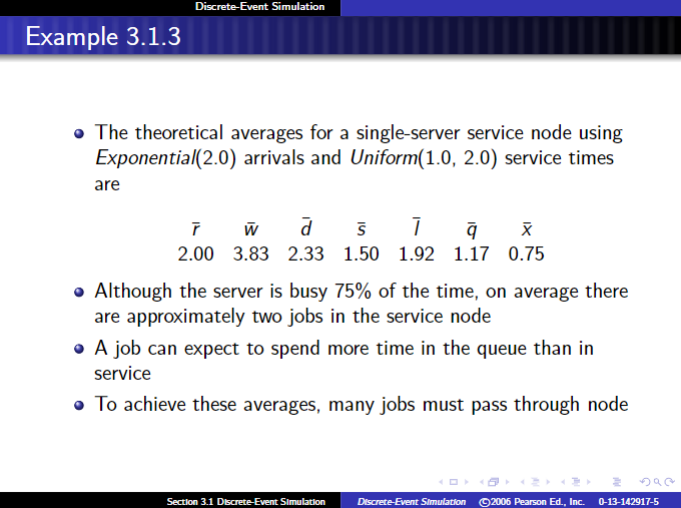
\includegraphics[scale=0.75]{Sections/Q2/3.1.3.png}\\
\vspace{10pt}
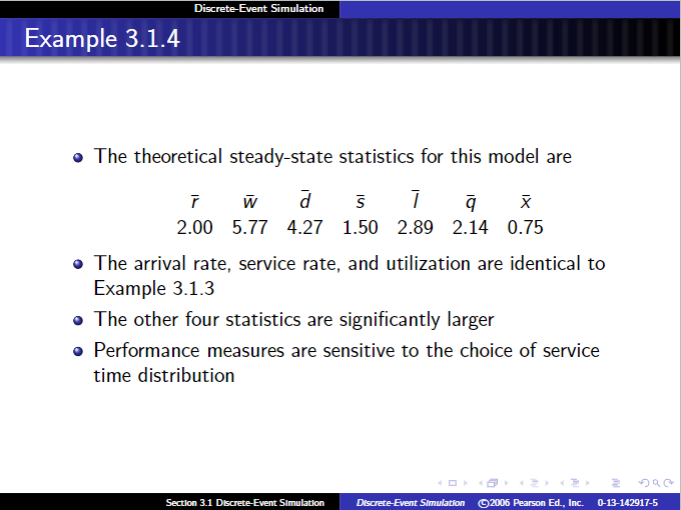
\includegraphics[scale=0.75]{Sections/Q2/3.1.4.png}\\
\end{center}
\newpage
\vspace{35pt}
\begin{center}
    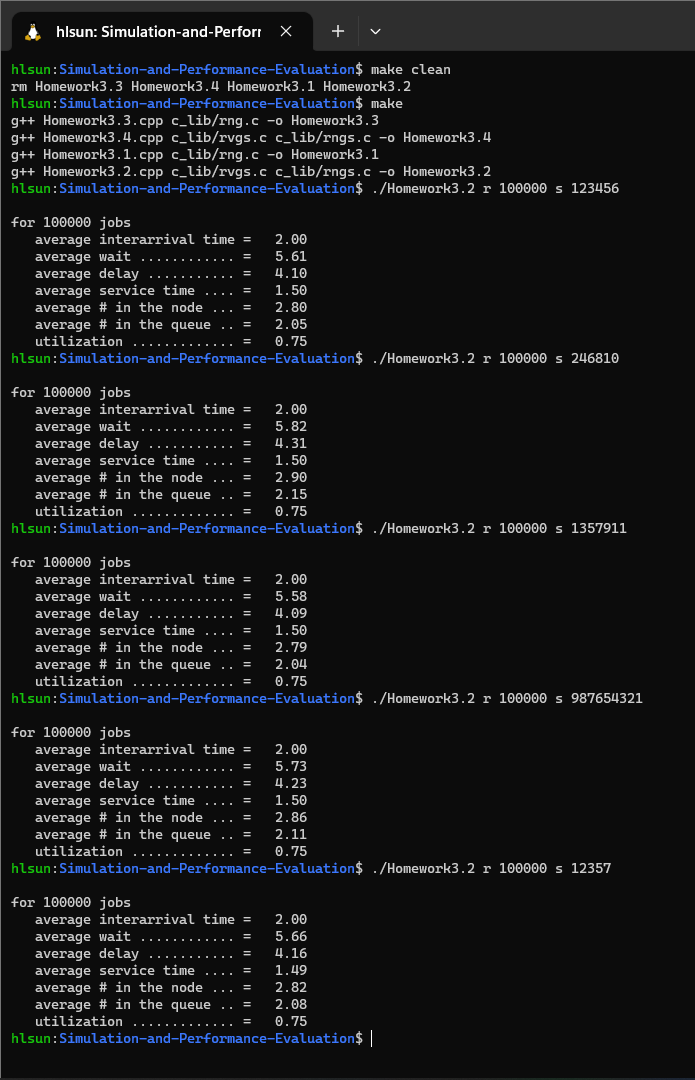
\includegraphics[scale=0.75]{Sections/Q2/H3_2.png}
\end{center}
\newpage
\begin{table}[h]
\centering
\begin{tabular}{l|lllll}
                  & 123456 & 246810 & 1357911 & 987654321 & 12357 \\
                  \hline\\
interarrival time & 2.00   & 2.00   & 2.00    & 2.00      & 2.00  \\
wait time         & 5.61   & 5.82   & 5.58    & 5.73      & 5.66  \\
delay time        & 4.10   & 4.31   & 4.09    & 4.23      & 4.16  \\
service time      & 1.50   & 1.50   & 1.50    & 1.50      & 1.49  \\
number in node    & 2.80   & 2.90   & 2.79    & 2.86      & 2.82  \\
number in queue   & 2.05   & 2.15   & 2.04    & 2.11      & 2.08  \\
utilization       & 0.75   & 0.75   & 0.75    & 0.75      & 0.75 
\end{tabular}
\end{table}
\noindent The arrival rate is the same because the interarrival time is defined by the same distribution as in Example 3.1.3: $r \sim Exponential(2.0)$.\\\\

\noindent The average service rate is the same as in Example 3.1.3 due to the distribution of the service times. The average number of tasks $\Bar{t}$ of $t \sim 1+ Geometric(0.9)$ is $1$ plus the inverse of $p=0.9$. Therefore, the average number of tasks is 10. The average of $Uniform(0.1, 0.2)$ is $0.15$. Multiplying this and the number of tasks together results in an average service rate $\Bar{s} = 1.5$, which is the same as the service rate in Example 3.1.3.\\\\

\noindent The server utilization is the same as in Example 3.1.3 because the average interarrival times and average service rates are the same in both examples. The server utilization is a ratio of the interarrival and service time averages.

\newpage
\begin{lstlisting}[style=CStyle]
/**
 * Homework 3.2
 * EECE 5643 - Simulation and Performance Evaluation
 * Author: Harrison Sun
 * Email: sun.har@northeastern.edu
 */

#include <cstdlib>
#include <cstring>
#include <stdio.h>
#include <exception>
#include <iostream>
#include <math.h> 
#include <string>
#include "c_lib/rvgs.h"
#include "c_lib/rngs.h"

#define LAST         10000L                   /* number of jobs processed */
#define START        0.0                      /* initial time             */

 /**
  * double GetArrival()
  *
  * @param void
  * @return arrival - the next arrival time
  *
  * This function calculates the arrival times for each process.
  */

double GetArrival()
{
    static double arrival = START;

    arrival += Exponential(2.0);
    return (arrival);
}


/**
 * double GetService()
 *
 * @param void
 * @return sum - the total service time for the process
 *
 * This function calculates the service times for each process.
 */

double GetService()
{
    long k{};
    double sum{ 0.0 };
    long tasks = 1 + Geometric(0.9);
    for (k = 0; k < tasks; ++k)
    {
        sum += Uniform(0.1, 0.2);
    }
    return sum;
}

/**
 * bool checkArg()
 *
 * @param char* input - the input string literal from the console
 * @return bool - true if the input is a number, false otherwise
 *
 * This function determines whether the argument is a number.
 */

bool checkArg(char* input)
{
    try
    {
        if (strlen(input) > 9)
        {
            throw std::logic_error("Number is too large.");
        }

        for (int i = 0; i < strlen(input); ++i)
        {

            if (std::isdigit(input[i])) continue;
            else
            {
                std::string errorMessage;
                errorMessage.append((std::string)input);
                errorMessage.append(" is not a digit.");
                throw std::logic_error(errorMessage);
            }
        }
        return 1;
    }

    catch (const std::logic_error& error)
    {
        std::cerr << error.what() << std::endl;
        return 0;
    }
}

/**
 * int main()
 *
 * @param int argc - the number of arguments
 * @param char* argv[] - the arguments
 *
 * @return int - 0 if the program runs successfully
 */

int main(int argc, char* argv[])
{
    long   index = 0;                         /* job index            */
    double arrival = START;                     /* time of arrival      */
    double delay;                                 /* delay in queue       */
    double service;                               /* service time         */
    double wait;                                  /* delay + service      */
    double departure = START;                     /* time of departure    */
    struct {                                      /* sum of ...           */
        double delay;                               /*   delay times        */
        double wait;                                /*   wait times         */
        double service;                             /*   service times      */
        double interarrival;                        /*   interarrival times */
    } sum = { 0.0, 0.0, 0.0 };

    long numRuns{};                                  /* number of runs */

    // Set the seed
    for (int i = 0; i < argc; ++i)
    {
        if (*argv[i] == 's' && checkArg(argv[i + 1]))
        {
            PutSeed(std::stol(argv[i + 1]));
            break;
        }
        else
        {
            PutSeed(123456789);
        }
    }

    // Set the number of runs
    for (int i = 0; i < argc; ++i)
    {
        if (*argv[i] == 'r' && checkArg(argv[i + 1]))
        {
            numRuns = std::stol(argv[i + 1]);
            break;
        }
        else
        {
            numRuns = 10000;
        }
    }

    while (index < numRuns) {
        index++;
        arrival = GetArrival();
        if (arrival < departure)
            delay = departure - arrival;         /* delay in queue    */
        else
            delay = 0.0;                         /* no delay          */
        service = GetService();
        wait = delay + service;
        departure = arrival + wait;              /* time of departure */
        sum.delay += delay;
        sum.wait += wait;
        sum.service += service;
    }
    sum.interarrival = arrival - START;

    printf("\nfor %ld jobs\n", index);
    printf("   average interarrival time = %6.2f\n", sum.interarrival / index);
    printf("   average wait ............ = %6.2f\n", sum.wait / index);
    printf("   average delay ........... = %6.2f\n", sum.delay / index);
    printf("   average service time .... = %6.2f\n", sum.service / index);
    printf("   average # in the node ... = %6.2f\n", sum.wait / departure);
    printf("   average # in the queue .. = %6.2f\n", sum.delay / departure);
    printf("   utilization ............. = %6.2f\n", sum.service / departure);
    return 0;
}
\end{lstlisting}
\textbf{\noindent (a) If these times are for an initially idle single-server FIFO service node with infinite capacity, calculate the average service time, the server's utilization, and the traffic intensity.}

\begin{lstlisting}[style=CStyle]
/**
 * Homework 2.2 
 * EECE 5643 - Simulation and Performance Evaluation
 * Author: Harrison Sun
 * Email: sun.har@northeastern.edu
 */

#include <iostream>
#include <vector>
#include <fstream>

/**
 * int main()
 * 
 ************* Terminal Arguments *************
 * @param int argc - number of arguments      *
 * @param char* argv[] - array of arguments   *
 **********************************************
 * 
 * @return 0 if successful
 * 
 * This is the main function. It reads in a data file in tab separated format. The first column contains the arrival times and the second column
 * contains departure times. This function calculates the average service time, the server utilization, and the traffic intensity.  
 */

int main(int argc, char* argv[])
{
    /* Read in the data file and store the arrival times and departure times as two vectors. */
    std::vector<double> arrival_times {};
    std::vector<double> departure_times {};

    std::ifstream infile = (argc > 1) ? std::ifstream(argv[1]) : std::ifstream("ac.dat");
    double arrival_time {};
    double departure_time {};
    while (infile >> arrival_time >> departure_time)
    {
        arrival_times.push_back(arrival_time);
        departure_times.push_back(departure_time);
    }

    /* Calculate the service time as departure time minus the start time of the job. */
    double total_service_time {};
    for (int i = 0; i < arrival_times.size(); ++i)
    {
        /* Check if the service node is free at arrival */
        if (arrival_times[i] > departure_times[i-1])
        {
            total_service_time += (departure_times[i] - arrival_times[i]);
        }
        /* If the job has to wait in a queue, the service starts after the previous job is finished */
        else
        {
            total_service_time += (departure_times[i] - departure_times[i-1]);
        }
    }

    /* Calculate the average service time */
    double average_service_time = total_service_time / arrival_times.size();

    /* Print the average service time */
    std::cout << "The average service time is: " << average_service_time << std::endl;

    /* Calculate the server utilization */
    /* Calculate the start time for each job. */
    double timeUtilized{0};
    for (int i = 0; i < arrival_times.size(); ++i)
    {
		/* Check if the service node is free at arrival */
		if (arrival_times[i] > departure_times[i - 1])
		{
			timeUtilized += departure_times[i] - arrival_times[i];
		}
		/* If the job has to wait in a queue, the service starts after the previous job is finished */
		else
		{
			timeUtilized += departure_times[i] - departure_times[i - 1];
		}
    }
    
    /* Divide the server utilization by the total amount of time the program is run. */
    timeUtilized /= departure_times[departure_times.size()-1];
    /* Print the server utilization time. */
    std::cout << "The server utilization is: " << timeUtilized << std::endl;
	
	/* Calculate the traffic intensity */
	/* The traffic intensity is calculated as the ratio of the interarrival rate to service rate. */
	/* Calculate the interarrival rate. */
    double interarrival_rate{ arrival_times[arrival_times.size() - 1] / arrival_times.size() };

    double trafficIntensity { average_service_time / interarrival_rate };

    std::cout << "The traffic intensity is: " << trafficIntensity << std::endl;
	
    return 0;
}
\end{lstlisting}
\newpage
\noindent Terminal Output:\\
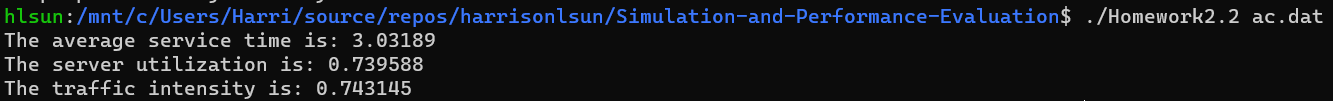
\includegraphics[scale=0.5]{Sections/H2_2.png}\\
The average service time is: 3.03189\\
The server utilization is: 0.739588\\
The traffic intensity is: 0.743145\\\\

\textbf{\noindent(b) Be explicit: For $i = 1,2,...,n$, how does $s_i$ related to $a_{i-1}$,$a_i$,$c_{i-1}$ and $c_i$?\\\\}
When $a_i$ is greater than $c_{i-1}$, this means that there is no delay before $a_i$ can start being processed. Thus, $s_i = c_i - a_i$. However, when $a_i$ is less than $c_{i-1}$, this means that job $i$ has to wait in the queue. Therefore, in this case, $s_i = c_i - c_{i-1}$. \\\\
\pagebreak

\section{\textbf{Ex. 2.3.4}}
\textbf{Suppose that each die in a pair of dice is loaded (unfair) in such a way that the
6-face is four times as likely as the opposite 1-face and each of the other four faces are twice as likely as the 1-face.\\\\}
\textbf{(a) Use Monte Carlo simulation to estimate the probability that, if the dice are rolled, the sum of the two up-faces will be 7.\\\\}
\begin{lstlisting}[style=CStyle]
/**
 * Homework 2.3
 * EECE 5643 - Simulation and Performance Evaluation
 * Author: Harrison Sun
 * Email: sun.har@northeastern.edu
 */

#define ONEFACEWEIGHT	1
#define OTHERWEIGHT		2
#define SIXFACEWEIGHT	4
#define DEFAULTSEED		0L
#define NUMRUNS			1000000L

#include <exception>
#include <iostream>
#include <stdlib.h>
#include "c_lib/rng.h"

/* Dice Weights */																																					
double oneFaceWeight{ ONEFACEWEIGHT };																																
double otherFaceWeight{ OTHERWEIGHT };																																
double sixFaceWeight{ SIXFACEWEIGHT };																														
/* TOTAL WEIGHT */																																					
double totalWeight{ oneFaceWeight + sixFaceWeight + 4 * otherFaceWeight };																							

/* Dice Probabilities */																																			
double p1 = oneFaceWeight / totalWeight;																															
double pOther = otherFaceWeight / totalWeight;																														
double p6 = sixFaceWeight / totalWeight;																																	
/* Define the thresholds */																																			
double threshold1 = p1;																																				
double threshold2 = threshold1 + pOther;																															
double threshold3 = threshold2 + pOther;																															
double threshold4 = threshold3 + pOther;																															
double threshold5 = threshold4 + pOther;																													
double threshold6 = threshold5 + p6;		/* threshold6 should be equal to 1 */	


/**
 * int Throw_Die(void)
 * 
 * @param void
 * 
 * @return int - the number of the face of the die
 * 
 * This function simulates the throwing of a die. It returns the number of the face of the die.
 */

int Throw_Die(void)
{
	/* Roll the die */
	double r = Random();
	int die{};
	if (r < threshold1)
	{
		die = 1;
	}
	else if (r < threshold2)
	{
		die = 2;
	}
	else if (r < threshold3)
	{
		die = 3;
	}
	else if (r < threshold4)
	{
		die = 4;
	}
	else if (r < threshold5)
	{
		die = 5;
	}
	else if (r < threshold6)
	{
		die = 6;
	}
	else
	{
		std::cerr << "Error: Random number is greater than 1." << std::endl;
		throw std::logic_error("My code is broken. This really shouldn't happen.");
	}
	return die;
}

/**
 * int main()
 * 
 ************* Terminal Arguments *************
 * @param int argc - number of arguments      *
 * @param char* argv[] - array of arguments   *
 **********************************************
 * 
 * @return int - 0 if successful
 * 
 * This is the main function. It uses a Monte Carlo Simulation to estimate the probability that, if weighted dice are rolled, the sum of the two up-faces will be 7.
 */

int main(int argc, char* argv[])
{
	/* Seed definition */
	long seed = (argc > 1) ? atol(argv[1]) : DEFAULTSEED;

	/* Number of runs */
	long num_runs = (argc > 2) ? atol(argv[2]) : NUMRUNS;
	
	/* Random Number Generator */
	PutSeed(seed);
	
	/* Number of times the sum of the two up-faces is 7 */
	long num_7{ 0 };

	/* Roll the dice twice and add the faces together */
	for (int i = 0; i < num_runs; ++i)
	{
		/* Try-Catch Block to catch exceptions (Sum(Pr) != 1) */
		try 
		{
			num_7 = (Throw_Die() + Throw_Die() == 7) ? ++num_7 : num_7;
		}
		catch (const std::logic_error& error)
		{
			std::cerr << error.what() << std::endl;
			return -1;
		}
	}

	/* Print the results */
	std::cout << "The probability that the sum of the two up-faces is 7 is " << (double)num_7 / num_runs << std::endl;

	return 0;
}
\end{lstlisting}
\vspace{50pt}
Terminal Outputs:\\\\
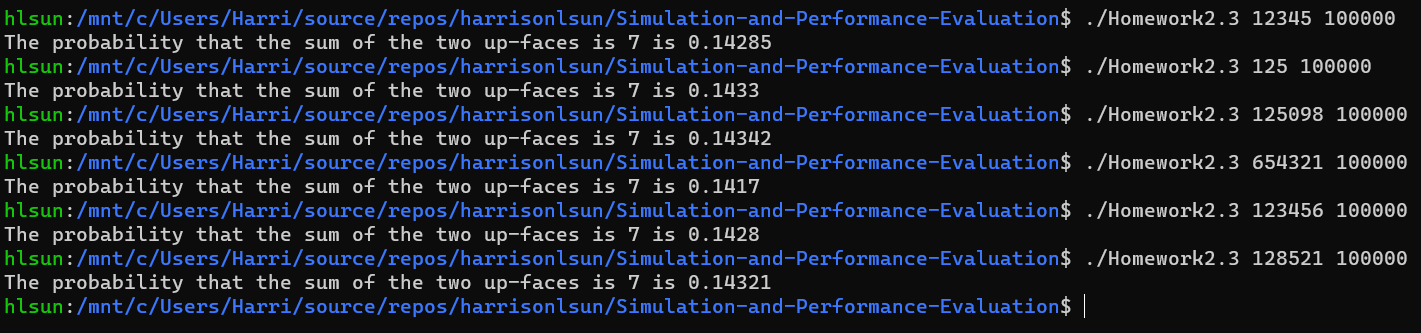
\includegraphics[scale=0.55]{Sections/H2_3.png}\\\\
\textbf{\newpage\noindent(b) What is the axiomatic probability?\\\\}
\begin{align*}
    &\text{Combination} &\text{Calculation}\hspace{100pt}  &\text{Probability}\\
    &\text{1 and 6 }&\frac{1}{13}\times \frac{4}{13}\hspace{100pt} &\frac{4}{169}\\
    &\text{2 and 5 }&\frac{4}{13}\times \frac{1}{13}\hspace{100pt} &\frac{4}{169}\\
    &\text{3 and 4 }&\frac{2}{13}\times \frac{2}{13}\hspace{100pt} &\frac{4}{169}\\
    &\text{4 and 3 }&\frac{2}{13}\times \frac{2}{13}\hspace{100pt} &\frac{4}{169}\\
    &\text{5 and 2 }&\frac{2}{13}\times \frac{2}{13}\hspace{100pt} &\frac{4}{169}\\
    &\text{6 and 1 }&\frac{4}{13}\times \frac{1}{13}\hspace{100pt} &\frac{4}{169}\\
    &\textbf{SUM} & \hspace{200pt} &\frac{24}{169} = 0.142 
\end{align*}

\noindent The axiomatic probability is 0.142.
\pagebreak

\section{\textbf{Ex. 2.3.5}}
\textbf{(a) If two points are selected at random on the circumference of a circle of
radius $\rho$, use Monte Carlo simulation to estimate the probability that the distance between the points is greater than $\rho$.\\\\}

\begin{lstlisting}[style=CStyle]
/**
 * Homework 2.4
 * EECE 5643 - Simulation and Performance Evaluation
 * Author: Harrison Sun
 * Email: sun.har@northeastern.edu
 */

#define defaultradius		1.0
#define defaultseed			0L
#define numruns				100000

#include <iostream>
#include <math.h>
#include <stdlib.h>
#include "c_lib/rng.h"

/**
 * int main()
 * 
 * @param int argc - the number of arguments
 * @param char* argv[] - the array of arguments
 * 
 * This is the main function. It randomly selects two points on the circumference of a circle and calculates the distance between them. 
 * This program calculates the probability that this distance is greater than the radius.
 */

int main(int argc, char* argv[])
{
	long seed = (argc > 1) ? atol(argv[1]) : defaultseed;
	double radius = (argc > 2) ? atof(argv[2]) : defaultradius;

	PutSeed(seed);
	
	int count{ 0 };
	
	for (int i = 0; i < numruns; ++i)
	{
		/* Find the angle of the point on the circle. */
		double angle1 = 2 * M_PI * Random();
		double angle2 = 2 * M_PI * Random();
		
		/* Distance Formula */
		double distance = sqrt(pow((radius * cos(angle1) - radius * cos(angle2)),2) + pow((radius * sin(angle1) - radius * sin(angle2)),2));
		count += (distance > radius) ? 1 : 0;
	}
	
	std::cout << "The probability that the distance between two points on the circumference of a circle is greater than the radius is "
		<< (double)count / numruns << std::endl;
	
	return 0;
}
\end{lstlisting}
\newpage \noindent
Terminal Outputs:\\
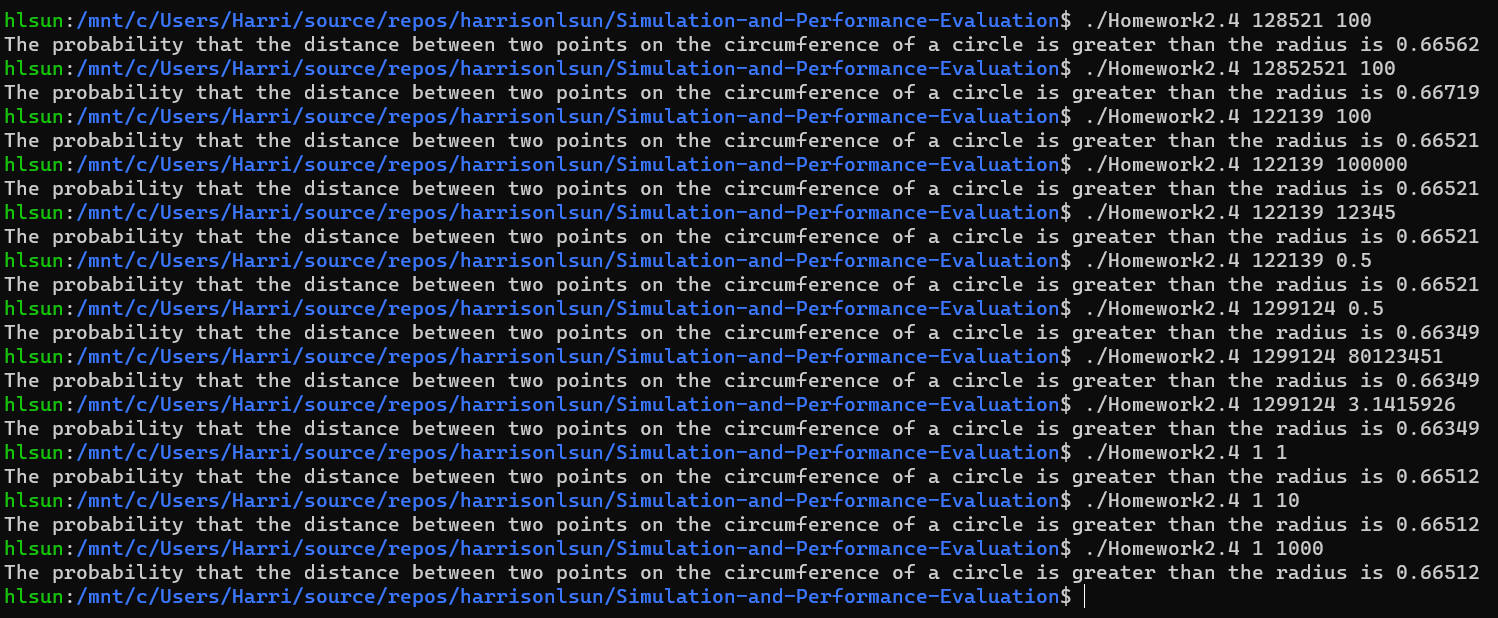
\includegraphics[scale=0.5]{Sections/H2_4.png}\\\\\\

\textbf{(b) How does this probability depend on $\rho$?\\\\}
It is not affected by $\rho$.\\\\
We can see from the Monte Carlo Simulation that the probability of the distance being greater than the radius is approximately $\frac{2}{3}$. Furthermore, this probability is unaffected by the radius at all and the values are exactly the same given the same seed. This is because the chord length, which we can denote as $\mathcal{L}$ is proportional to the radius $\rho$ such that $\mathcal{L} = 2\times\rho\times sin(\frac{\theta}{2})$ where $\theta$ is the minor angle of the chord. We can represent this as any given point fixed in space on the circumference of the circle and the other point rotated about the center of the circle given by $\theta$ in either direction. Given this, we can say that we can consider a single direction and limit the angle to $\theta \leq \pi$. $\mathcal{L} > \rho $ when $sin(\frac{\theta}{2}) \geq \frac{1}{2}$. Thus, this occurs so long as $\theta \geq \frac{\pi}{3}$. Remembering that $\theta \sim  Uniform[0, \pi]$, this means that $\frac{2}{3}$ of the time, the length of the chord will be greater than the radius irrelevant of what the radius is.\\\\
\end{document}
